\documentclass[a4paper,10pt]{article}
% - a4paper: printing paper format
% - 10pt: size of the characters

\usepackage{graphicx}
\usepackage{titling}
\usepackage{listings}
\usepackage[table]{xcolor}
\newcolumntype{R}[1]{>{\raggedleft\arraybackslash }b{#1}}
\newcolumntype{L}[1]{>{\raggedright\arraybackslash }b{#1}}
\newcolumntype{C}[1]{>{\centering\arraybackslash }b{#1}}
\lstset{%
  basicstyle=\scriptsize\sffamily,%
  commentstyle=\footnotesize\ttfamily,%
  frameround=trBL,
  frame=single,
  breaklines=true,
  showstringspaces=false,
  numbers=left,
  numberstyle=\tiny,
  numbersep=10pt,
  keywordstyle=\bf
}
\newcommand{\subtitle}[1]{%
  \posttitle{%
    \par\end{center}
    \begin{center}\large#1\end{center}
    \vskip0.5em}%
}



%%%%%%%%%%%%%%%%%%%%%%%%%%%%%%%%%%%%%%%%%%%%%%%%%%%%
%				Title / Subtitle / Authors and Date									   %
% This should be adapted to your report.					                                                              %
%																			   %
%%%%%%%%%%%%%%%%%%%%%%%%%%%%%%%%%%%%%%%%%%%%%%%%%%%%
\title{TD3 : Formatted I/O Library}
\subtitle{Master M1 MOSIG, Grenoble Universities}
\author{Lenka Kun\'{i}kov\'{a} \and Lina Marsso}
\date{26/10/2014}

\begin{document}
% Beginning serious stuff. 


\maketitle
% Actually prints title / subtitle / authors and dat into the document


%%%%%%%%%%%%%%%%%%%%%%%%%%%%%%%%%%%%%%%%%%%%%%%%%%%%
%								Abstract										   %
% Change the part below the abstract so that it corresponds to your report	                                     %
%																			   %
%%%%%%%%%%%%%%%%%%%%%%%%%%%%%%%%%%%%%%%%%%%%%%%%%%%%

%%%%%%%%%%%%%%%%%%%%%%%%%%%%%%%%%%%%%%%%%%%%%%%%%%%%
%								Introductio	n									   %
%																			   %
% the command \section{name of the section} begins a new section of the document                            %
%																			   %
%%%%%%%%%%%%%%%%%%%%%%%%%%%%%%%%%%%%%%%%%%%%%%%%%%%%
\section{Introduction}
	\paragraph{}
	In this project we have to implement a I/O  library. 
	And evaluate their performances in different applications.
	\paragraph{}
	Firstly in this report we give answers of questions in the subject. 
	Then we present you our implementation.
	Then we speak about the safety checks implementation. 
	Finnaly, we analyse the performance and conclude this project.

\section{Subject questions}
\subsection{Question 1}


\section{Implementation}	
\begin{enumerate}
\item We initialize the memory with the function memory\_init
\item We alloc the new block with mem\_alloc like that~:
	\begin{itemize}
	\item We find the address of new block allocated with one between
	 the strategy 3
	(First fit, Worse fit, best fit). We can choose. Basically, it's first fit.
	\item We allocate the full block and update list of freeblock
	\end{itemize}
\item We can free a block with free\_block~:
	\begin{itemize}
	\item We find an adjacent block to the one to be freed and try to merge then
	\item If no adjacent block~:~create a new block and insert it in the list
	\end{itemize}
\end{enumerate}
 
\section{Safety checks}

\section{Evaluation}
\paragraph{}
For evaluate our library, we use one test he copie one file in an
other file buffered for our library and we write the same test 
but using the standard open, read and write.
\paragraph{}
We evaluate in the begining the time for copy two file with our library, 
and with the standard open, read and write. We have also one ratio~: 
\begin{equation}
\left(\frac{My\_stdio\_time\_execution}{Standar\_Read\_Write\_time\_execution} \right)  \quad
\end{equation}
\paragraph{}
We calculate the time of the execution with a script time.sh. We can see

\begin{tabular}{|R{2cm}|C{2cm}|L{1.5cm}|L{1.5cm}|}
\hline \rowcolor{lightgray}Library & Time (microsecondes) & Size of file\\
\hline  libmy\_sdio & 4 & 8.0K \\
\hline  Standar  & 36 & 8.0K \\
\hline 
\end{tabular}

\begin{figure}[ht]
\center 
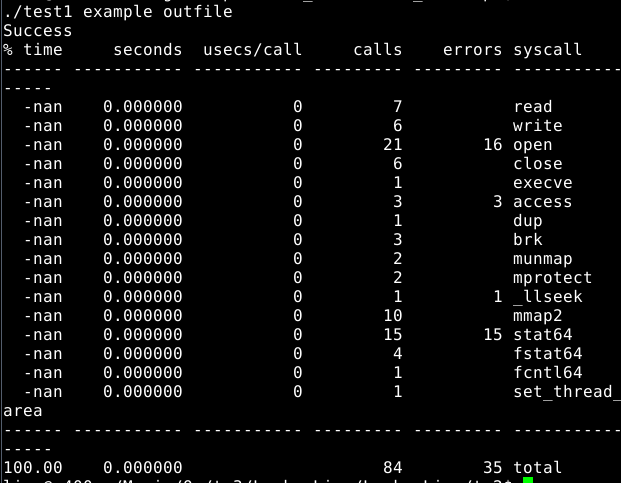
\includegraphics[width=0.85\linewidth]{my_strace.png}
\caption{Number of system call of our library}
\label{first}
\end{figure}
\begin{figure}[ht]
\center 
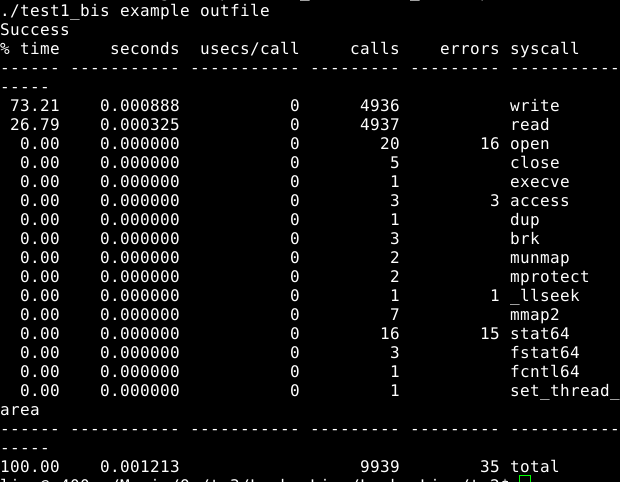
\includegraphics[width=0.85\linewidth]{syscall_strace.png}
\caption{Number of system call with read and write}
\label{worst}
\end{figure}
\begin{figure}[ht]
\center 
%\includegraphics[width=0.8\linewidth]{gcc_best_fit.png}
\caption{Memory requested and memory used with best fit strategy}
\label{best}
\end{figure}

\subsection{Table with fragmentation level of differents programs}

\begin{tabular}{|R{2cm}|C{1.5cm}|L{1.5cm}|L{1.5cm}|}
\hline \rowcolor{lightgray}program & worst\_fit & best\_fit & first\_fit \\
\hline  ls & 1.83 & 1.83 & 2.48 \\
\hline  wc & 0.96 & 0.96 & 0.96 \\
\hline  ps & 1.37 & 1.36 & 1.37 \\
\hline  hostname & 2.42 & 2.42 & 3.23 \\
\hline 
\end{tabular}

\section{Conclusion}
\paragraph{}
The goal of this project was to get familiar with the concept of memory 
managment and I think we succeeded. We managed to implement a simple 
version of memory allocator which allows users to allocate and free memory.
\paragraph{} 
During the implementation we had to deal with several problems. For 
example we needed to find a way on how to determine positions of free 
blocks when we do not have linked lists of them, or think about the 
algorithm that helps us merge contiguous blocks of free space. Moreover, 
we implemented the three most common algorithms for finding an appropriate 
free block (first-fit, best-fit and worse-fit). We are now able to describe 
pros and cons for each of them.
\paragraph{}
In the second part, we added some other features to our memory allocator. 
All of them related to security checks. Now we know that implementing 
functions for free and alloc memory is not enough and we also need 
to deal with situations where users (on purpose or by chance) do not act the 
way we expect. The control we are making is not perfect but it helps 
us to deal with many cases that may happen.

\paragraph{}
Finnaly, we can see an application of our allocator. We can analyse it's
performance with many apllications like ls, hostname... It was a very 
interesting project.

 \end{document}
